%Set Aspect Ratio%
\documentclass[aspectratio = 169]{beamer}

\usetheme{CambridgeUS}

%For 'TM' Symbol used later
\usepackage{textcomp}

%Set Button Colour%
\setbeamercolor{button}{bg=gray,fg=white}

%Disable the Navigation Tools%
\beamertemplatenavigationsymbolsempty

\setbeamertemplate{footline}[frame number]{}

%Metadata%
\title{Expediting the Document Formatting Process}
\author{Jeremy Hall Spence \\ Department of Media, Music, Communication and Cultural Studies}
\date{This presentation is available at: \\ \href{https://github.com/JeremyHallSpence/PICO}{\underline{https://github.com/JeremyHallSpence/PICO}}}

%Set Space Between Paragraphs%
\setlength{\parskip}{1em}



\begin{document}

%TITLE

\begin{frame}

\maketitle

\end{frame}



%INTRODUCTION I%

\begin{frame}
\label{introI}
\frametitle{Typesetting}

\begin{columns}

\column{0.15\textwidth}

\hyperlink{introI}{\beamerbutton{Introduction I}} \newline
\hyperlink{introII}{\beamerbutton{Introduction II}} \newline 
\hyperlink{scoping}{\beamerbutton{Scoping}} \newline
\hyperlink{elaboration}{\beamerbutton{Elaboration}} \newline  
\hyperlink{software}{\beamerbutton{Software}} \newline 
\hyperlink{toolchain}{\beamerbutton{Tool Chain}} \newline 
\hyperlink{learning}{\beamerbutton{Learning}} \newline 
\hyperlink{problems}{\beamerbutton{Problems}} \newline 
\hyperlink{results}{\beamerbutton{Results}} \newline
\hyperlink{exampleI}{\beamerbutton{Example I}} \newline 
\hyperlink{exampleII}{\beamerbutton{Example II}}  

\column{0.8\textwidth}

\begin{center}
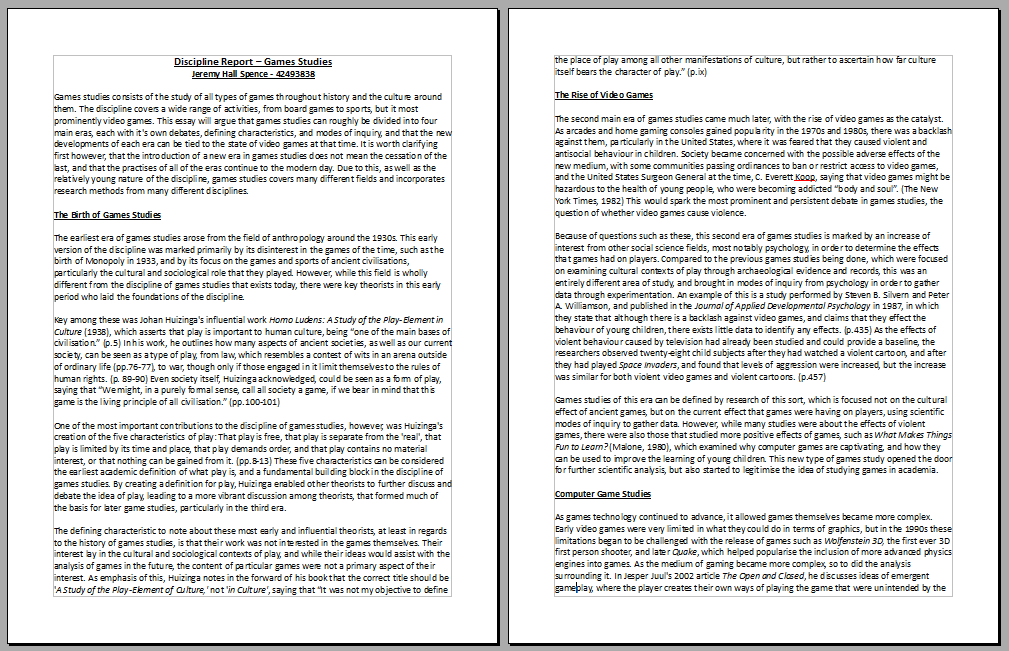
\includegraphics[scale = 0.4]{untypeset}
\end{center}

\end{columns}
\end{frame}



%INTRODUCTION II%

\begin{frame}
\label{introII}
\frametitle{Typesetting}

\begin{columns}

\column{0.15\textwidth}


\hyperlink{introI}{\beamerbutton{Introduction I}} \newline
\hyperlink{introII}{\beamerbutton{Introduction II}} \newline 
\hyperlink{scoping}{\beamerbutton{Scoping}} \newline
\hyperlink{elaboration}{\beamerbutton{Elaboration}} \newline  
\hyperlink{software}{\beamerbutton{Software}} \newline 
\hyperlink{toolchain}{\beamerbutton{Tool Chain}} \newline 
\hyperlink{learning}{\beamerbutton{Learning}} \newline 
\hyperlink{problems}{\beamerbutton{Problems}} \newline 
\hyperlink{results}{\beamerbutton{Results}} \newline
\hyperlink{exampleI}{\beamerbutton{Example I}} \newline 
\hyperlink{exampleII}{\beamerbutton{Example II}}  


\column{0.8\textwidth}

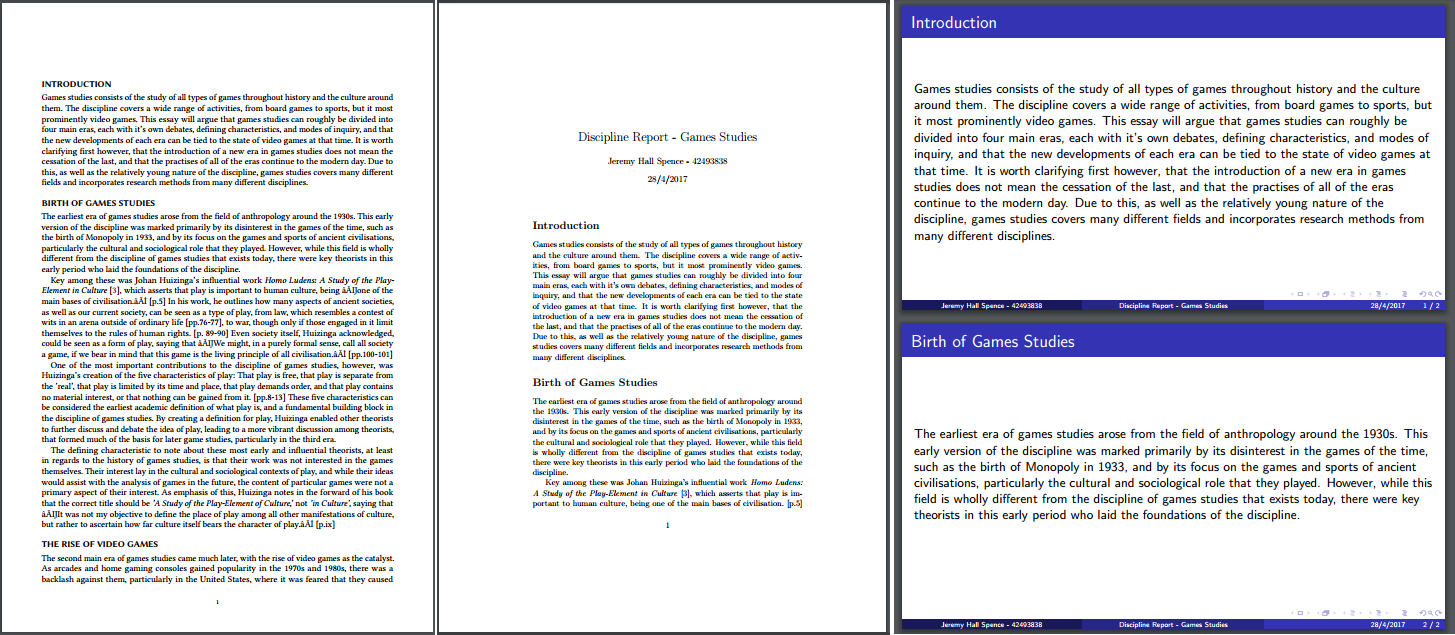
\includegraphics[scale = 0.3]{typeset}

\end{columns}
\end{frame}



%SCOPING%

\begin{frame}
\label{scoping}
\frametitle{Scoping}
\begin{columns}

\column{0.15\textwidth}


\hyperlink{introI}{\beamerbutton{Introduction I}} \newline
\hyperlink{introII}{\beamerbutton{Introduction II}} \newline 
\hyperlink{scoping}{\beamerbutton{Scoping}} \newline
\hyperlink{elaboration}{\beamerbutton{Elaboration}} \newline  
\hyperlink{software}{\beamerbutton{Software}} \newline 
\hyperlink{toolchain}{\beamerbutton{Tool Chain}} \newline 
\hyperlink{learning}{\beamerbutton{Learning}} \newline 
\hyperlink{problems}{\beamerbutton{Problems}} \newline 
\hyperlink{results}{\beamerbutton{Results}} \newline
\hyperlink{exampleI}{\beamerbutton{Example I}} \newline 
\hyperlink{exampleII}{\beamerbutton{Example II}}  


\column{0.8\textwidth}

While I was undecided about what my research would entail in the second year of my degree, the one one certainty would be the amount of writing involved.
\\~\\
Therefore, I decided that my project would be the creation of a tool chain to simplify my thesis writing. This tool chain would be designed to produce professional looking documents and automatically handle referencing, while also speeding up the writing process. As a test of this tool chain, my proof-of-concept would be to format a document to meet Macquarie University's thesis requirements.

\end{columns}
\end{frame}



%ELABORATION%
\begin{frame}
\label{elaboration}
\frametitle{Elaboration}
\begin{columns}

\column{0.15\textwidth}


\hyperlink{introI}{\beamerbutton{Introduction I}} \newline
\hyperlink{introII}{\beamerbutton{Introduction II}} \newline 
\hyperlink{scoping}{\beamerbutton{Scoping}} \newline
\hyperlink{elaboration}{\beamerbutton{Elaboration}} \newline  
\hyperlink{software}{\beamerbutton{Software}} \newline 
\hyperlink{toolchain}{\beamerbutton{Tool Chain}} \newline 
\hyperlink{learning}{\beamerbutton{Learning}} \newline 
\hyperlink{problems}{\beamerbutton{Problems}} \newline 
\hyperlink{results}{\beamerbutton{Results}} \newline
\hyperlink{exampleI}{\beamerbutton{Example I}} \newline 
\hyperlink{exampleII}{\beamerbutton{Example II}}  


\column{0.8\textwidth}

To meet the goal of my proof-of-concept, I first found the style requirements for a Macquarie University thesis, available \href{http://www.hdr.mq.edu.au/information\_for/current\_candidates/thesis\_preparation\#presentation}{\underline{here}}. These requirements are:

\begin{itemize}
\item Double or one and a half sized spacing
\item A 3.5cm margin on the binding edge
\item A 1.5cm margin on all other edges
\item Numbered pages
\item A title page, table of contents, and 200 word summary
\end{itemize}

\end{columns}
\end{frame}



%SOFTWARE%

\begin{frame}
\label{software}
\frametitle{Software}
\begin{columns}

\column{0.15\textwidth}

\hyperlink{introI}{\beamerbutton{Introduction I}} \newline
\hyperlink{introII}{\beamerbutton{Introduction II}} \newline 
\hyperlink{scoping}{\beamerbutton{Scoping}} \newline
\hyperlink{elaboration}{\beamerbutton{Elaboration}} \newline  
\hyperlink{software}{\beamerbutton{Software}} \newline 
\hyperlink{toolchain}{\beamerbutton{Tool Chain}} \newline 
\hyperlink{learning}{\beamerbutton{Learning}} \newline 
\hyperlink{problems}{\beamerbutton{Problems}} \newline 
\hyperlink{results}{\beamerbutton{Results}} \newline
\hyperlink{exampleI}{\beamerbutton{Example I}} \newline 
\hyperlink{exampleII}{\beamerbutton{Example II}}  


\column{0.8\textwidth}

I would also need to choose the typesetting software and bibliography management software that I would incorporate into my tool chain. LaTeX, ConTeXt and Adobe InDesign\texttrademark, were the most widely used typesetting programs, and all could handle the requirements. I chose LaTeX due to InDesign's price, and ConTeXt's difficulty to install on Windows.
\\~\\
For bibliography management software, I chose Mendeley because it can export .bib files, which LaTeX can use to automatically create a bibliography and in-text citations.

\end{columns}
\end{frame}



%TOOLCHAIN

\begin{frame}
\label{toolchain}
\frametitle{Tool Chain}
\begin{columns}

\column{0.15\textwidth}

\hyperlink{introI}{\beamerbutton{Introduction I}} \newline
\hyperlink{introII}{\beamerbutton{Introduction II}} \newline 
\hyperlink{scoping}{\beamerbutton{Scoping}} \newline
\hyperlink{elaboration}{\beamerbutton{Elaboration}} \newline  
\hyperlink{software}{\beamerbutton{Software}} \newline 
\hyperlink{toolchain}{\beamerbutton{Tool Chain}} \newline 
\hyperlink{learning}{\beamerbutton{Learning}} \newline 
\hyperlink{problems}{\beamerbutton{Problems}} \newline 
\hyperlink{results}{\beamerbutton{Results}} \newline
\hyperlink{exampleI}{\beamerbutton{Example I}} \newline 
\hyperlink{exampleII}{\beamerbutton{Example II}}  


\column{0.8\textwidth}
\begin{figure}
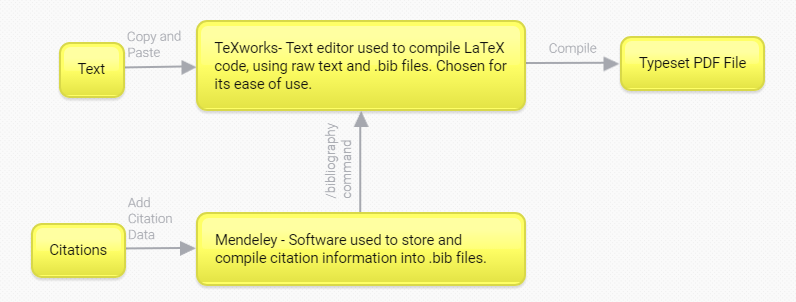
\includegraphics[scale = 0.45]{toolchain}
\caption{The Proof-of-Concept Tool Chain}
\end{figure}
Text is copied straight from a Word document to intergrate with the LaTeX code in TeXworks. Citation data is exported from Mendeley into a .bib file, which is them be called upon in the LaTeX code in TeXworks. The .pdf document can then be compiled.
\end{columns}
\end{frame}



%LEARNING%

\begin{frame}
\label{learning}
\frametitle{Learning LaTeX}
\begin{columns}

\column{0.15\textwidth}

\hyperlink{introI}{\beamerbutton{Introduction I}} \newline
\hyperlink{introII}{\beamerbutton{Introduction II}} \newline 
\hyperlink{scoping}{\beamerbutton{Scoping}} \newline
\hyperlink{elaboration}{\beamerbutton{Elaboration}} \newline  
\hyperlink{software}{\beamerbutton{Software}} \newline 
\hyperlink{toolchain}{\beamerbutton{Tool Chain}} \newline 
\hyperlink{learning}{\beamerbutton{Learning}} \newline 
\hyperlink{problems}{\beamerbutton{Problems}} \newline 
\hyperlink{results}{\beamerbutton{Results}} \newline
\hyperlink{exampleI}{\beamerbutton{Example I}} \newline 
\hyperlink{exampleII}{\beamerbutton{Example II}}  
 

\column{0.8\textwidth}
While the initial learning curve for LaTeX was somewhat difficult, once I had established a basic understanding of the core principles it became quite easy to understand. In addition, LaTeX offers tutorials for beginners, and the online community is large and supportive.
\\~\\
Once I understood the basics, I was able to quickly change documents from one format to another by altering only a few lines of code. What was more difficult was making small adjustments, usually do do with layout, such as creating buttons in presentations.

\end{columns}
\end{frame}



%PROBLEMS%

\begin{frame}
\label{problems}
\frametitle{Problems}
\begin{columns}

\column{0.15\textwidth}

\hyperlink{introI}{\beamerbutton{Introduction I}} \newline
\hyperlink{introII}{\beamerbutton{Introduction II}} \newline 
\hyperlink{scoping}{\beamerbutton{Scoping}} \newline
\hyperlink{elaboration}{\beamerbutton{Elaboration}} \newline  
\hyperlink{software}{\beamerbutton{Software}} \newline 
\hyperlink{toolchain}{\beamerbutton{Tool Chain}} \newline 
\hyperlink{learning}{\beamerbutton{Learning}} \newline 
\hyperlink{problems}{\beamerbutton{Problems}} \newline 
\hyperlink{results}{\beamerbutton{Results}} \newline
\hyperlink{exampleI}{\beamerbutton{Example I}} \newline 
\hyperlink{exampleII}{\beamerbutton{Example II}}  


\column{0.8\textwidth}

The primary problem for my project was time management. I would have to learn and integrate two entirely new programs in only a few weeks. I attempted to minimize the time required by identifying what was essential for my project, and focusing my attention on learning that.
\\~\\
One other major problem was that for a few weeks I was unable to integrate the .bib files from Mendeley into LaTeX, which was a crucial step in my proposed workflow process. This problem was a result of my poor understanding of LaTeX, and was fixed with practice and further learning.

\end{columns}
\end{frame}



%RESULTS%

\begin{frame}
\label{results}
\frametitle{Results}
\begin{columns}

\column{0.15\textwidth}

\hyperlink{introI}{\beamerbutton{Introduction I}} \newline
\hyperlink{introII}{\beamerbutton{Introduction II}} \newline 
\hyperlink{scoping}{\beamerbutton{Scoping}} \newline
\hyperlink{elaboration}{\beamerbutton{Elaboration}} \newline  
\hyperlink{software}{\beamerbutton{Software}} \newline 
\hyperlink{toolchain}{\beamerbutton{Tool Chain}} \newline 
\hyperlink{learning}{\beamerbutton{Learning}} \newline 
\hyperlink{problems}{\beamerbutton{Problems}} \newline 
\hyperlink{results}{\beamerbutton{Results}} \newline
\hyperlink{exampleI}{\beamerbutton{Example I}} \newline 
\hyperlink{exampleII}{\beamerbutton{Example II}}  


\column{0.8\textwidth}

Despite these problems, my proof-of-concept was completed in time, and the repository containing my project can be found here: \\~\\ \href{https://github.com/JeremyHallSpence/Proof-of-Concept}{\underline{https://github.com/JeremyHallSpence/Proof-of-Concept}}
\\~\\
I successfully used the tool chain I had created to format an essay written earlier in the semester. References were gathered and exported from Mendeley in the form of .bib files, and text was copied into a template I had created using LaTeX. From there, I was able to export a .pdf file with formatting that met the requirements of Macquarie University, with references that were automatically generated.

\end{columns}
\end{frame}



% EXAMPLE I%

\begin{frame}
\label{exampleI}
\frametitle{Typesetting Example}
\begin{columns}

\column{0.15\textwidth}

\hyperlink{introI}{\beamerbutton{Introduction I}} \newline
\hyperlink{introII}{\beamerbutton{Introduction II}} \newline 
\hyperlink{scoping}{\beamerbutton{Scoping}} \newline
\hyperlink{elaboration}{\beamerbutton{Elaboration}} \newline  
\hyperlink{software}{\beamerbutton{Software}} \newline 
\hyperlink{toolchain}{\beamerbutton{Tool Chain}} \newline 
\hyperlink{learning}{\beamerbutton{Learning}} \newline 
\hyperlink{problems}{\beamerbutton{Problems}} \newline 
\hyperlink{results}{\beamerbutton{Results}} \newline
\hyperlink{exampleI}{\beamerbutton{Example I}} \newline 
\hyperlink{exampleII}{\beamerbutton{Example II}}  


\column{0.8\textwidth}

\begin{figure}
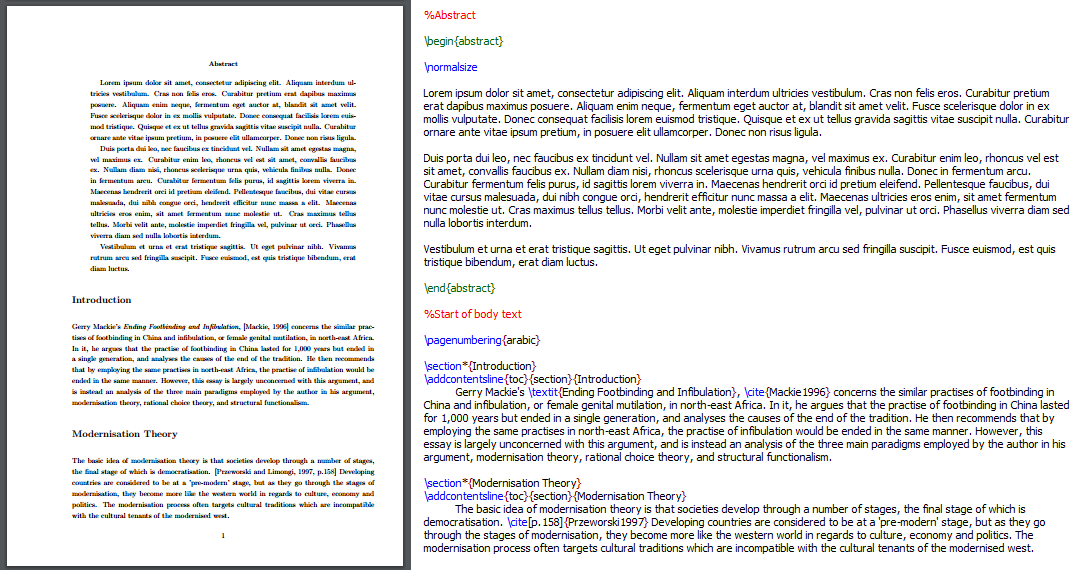
\includegraphics[scale = 0.35]{example1}
\caption{A section of the typeset document, and the code used to create that section.}
\end{figure}

\end{columns}
\end{frame}



%EXAMPLE II%

\begin{frame}
\label{exampleII}
\frametitle{Referencing Example}
\begin{columns}

\column{0.15\textwidth}

\hyperlink{introI}{\beamerbutton{Introduction I}} \newline
\hyperlink{introII}{\beamerbutton{Introduction II}} \newline 
\hyperlink{scoping}{\beamerbutton{Scoping}} \newline
\hyperlink{elaboration}{\beamerbutton{Elaboration}} \newline  
\hyperlink{software}{\beamerbutton{Software}} \newline 
\hyperlink{toolchain}{\beamerbutton{Tool Chain}} \newline 
\hyperlink{learning}{\beamerbutton{Learning}} \newline 
\hyperlink{problems}{\beamerbutton{Problems}} \newline 
\hyperlink{results}{\beamerbutton{Results}} \newline
\hyperlink{exampleI}{\beamerbutton{Example I}} \newline 
\hyperlink{exampleII}{\beamerbutton{Example II}}  


\column{0.8\textwidth}

\begin{figure}
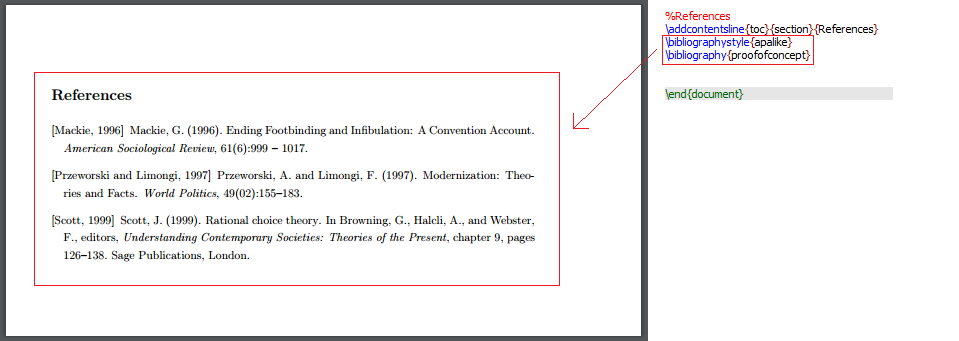
\includegraphics[scale = 0.5]{example2}
\caption{Using the two highlighted commands, LaTeX accesses the file in which bibliographic information is compiled, and automatically creates a list of references in the style specified.} 
\end{figure}

\end{columns}
\end{frame}



\end{document}